% !TeX root = Bericht.tex
% !TeX spellcheck = de_DE
\section{Ergebnisse}
Im gesamten Versuch wurde die Strahlungsintensität in Abhängigkeit von diversen Parametern untersucht. Die Intensität lässt sich dabei über ein Geiger-Müller Zählrohr (GMZ) ermitteln, welches Ionisierungsereignisse \( N \) misst. Diese folgen der Poisson Statistik, weshalb der Fehler auf \( \delta N = \sqrt{N} \) gesetzt wurde. Diverse Parameter des GMZ und der Röntgenquelle können über eine Software eingestellt werden und werden als Fehlerfrei angenommen. 

Bevor wir mit dem GMZ das Absorptionsverhalten diverser Materialien untersuchen, wollen wir dieses noch charakterisieren. Dafür wurde das Zählrohr auf \ang{5.5} geneigt, um eine Sättigung durch direktes Einstrahlen zu verhindern, und die Spannung von \( 300 \unit{V} \) bis \( 500 \unit{V} \) erhöht. Dabei wurden die Schritte so gewählt, dass Bereiche mit einer großen Änderung von \( N \) besser aufgelöst sind. Für jede Spannung wurden drei Werte händisch notiert, über die wir dann mitteln. Der Poisson Fehler wird dann nach der Mittlung angewendet. In \autoref{fig:Ex1} sind die gemessenen Zählraten $N$ auf die Zählrohrspannung $U$ aufgetragen. Zusätzlich wurde eine Exponentialfunktion an die rot markierten Datenpunkte gefittet, da diese optisch passt und sich Werte, wie Betriebsspannung, leicht ermitteln lassen.

\begin{figure}[H]
	\centering
	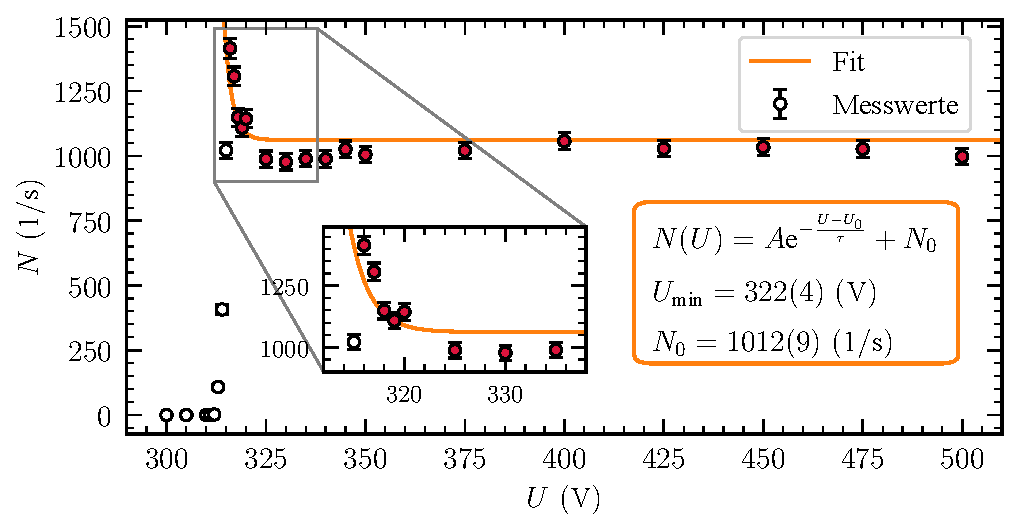
\includegraphics[width=\textwidth]{Ex1}
	\caption{Die gemessene Zählrate \( N \) ist auf die Wellenlänge \( \lambda \) aufgetragen. Die Daten sind mit poissonschem \( 1\sigma \) Unsicherheit angegeben. An rot markierte Datenpunkte wurde eine Exponentialfunktion angepasst, um die Betriebsspannung zu bestimmen. Die ermittelten Werte sind in der Ecke rechts unten zu sehen.}
	\label{fig:Ex1}
\end{figure}

In \autoref{fig:Ex1} lässt sich die Zählrohrcharakteristik des GMZ gut erkennen. Zählereignisse finden zunächst aufgrund zu geringer Spannung nicht statt, nehmen dann schnell zu und pendeln sich dann zu einen konstanten Wert ein. Die untere Grenze des Plateaubereichs wurde da gesetzt, wo die angepasste Exponentialfunktion nur mehr \( 1\% \) über dem konstanten Offset \( N_0 \) liegt (\( U_{\text{min}} = U_0 + \tau\log\left( A/0.01N_0 \right) = 322(4) \unit{V} \)). Der Überschuss der Zählereignisse vor dem Plateau wird wahrscheinlich durch Mehrfachzählung eines Ionisierungsereignisses verursacht. 

Jetzt wo der Arbeitsbereich des GMZ bekannt ist, wird dieser für die restlichen Messungen auf \( 500 \unit{V} \) gesetzt. Das kontinuierliche Röntgenspektrum lässt sich durch Einführen eines \ch{LiF} Kristalls mit Gitterebenenabstand \( d = 201 \unit{pm} \) ausmessen. Dabei wird der Winkel zwischen Kristallebene (an welcher Reflexion stattfindet) und GMZ von \ang{5.5} bis \ang{35} in \ang{0.1} Schritten verändert. Dabei wird das kontinuierliche Spektrum für festen Winkel dank der Bragg Reflexion nach einzelnen Wellenlängen gefiltert (siehe \autoref{bragg_schema}). In \autoref{fig:Ex2} ist das gemessene Spektrum auf die Wellenlänge, sowie Energie aufgetragen.

\begin{figure}[H]
	\centering
	\adjincludegraphics[width=\textwidth, clip, trim = {0 {.15\height} 0 {.15\height}}]{Ex2}
	\caption{Die gemessene Zählrate \( N \) ist auf die Wellenlänge \( \lambda \) aufgetragen. Die Energie der Photonen lässt sich aus der Wellenlänge bestimmen und ist als zweite x-Achse an der oberen Kante zu sehen. Die Daten sind mit poissonschem \( 1\sigma \) Unsicherheit angegeben, wobei diese zu klein ist um ausgemacht werden zu können. An die Daten wurde in orange eine Kombination aus drei Lorentz und einer linearen Funktion angepasst. Aus dem Fit lässt sich die Position der Peaks bestimmen, was links neben dem jeweiligen Peak vorgemerkt ist.}
	\label{fig:Ex2}
\end{figure}

Man kann in \autoref{fig:Ex2} einen kontinuierlichen Hintergrund mit drei prominenten Peaks erkennen. Letztere stammen von K Übergängen in der Anode. %(see \autoref{}).
Um die Energie der atomaren Übergänge zu bestimmen, wurde eine Multilorentz Funktion an die Daten angepasst und ist in orange zu sehen. Diese besteht aus der Summe von drei unabhängigen Lorentz Funktionen, auf welche ein konstanter Hintergrund addiert wurde. Aus dem Fit lassen sich Übergangsenergien zu
\begin{equation*}
	E_1 = 8.41(7) \unit{keV} \qquad E_2 = 9.7(2) \unit{keV} \qquad E_3 = 11.4(2) \unit{keV}
\end{equation*}
bestimmen, wobei als Fehler die Halbwertsbreite der Lorentz-Funktionen gewählt wurde. Die Literaturwerte für die Energie der Peaks betragen \autocite{SpektrumWolfram}
\begin{equation*}
	E_{L_{\alpha 1}} = 8.39 \unit{keV} \qquad E_{L_{\beta 1}} = 9.67 \unit{keV} \qquad E_{L_{\gamma 1}} = 11.28(2) \unit{keV} \qquad E_{L_{\gamma 2}} = 11.6 \unit{keV} 
\end{equation*}
Dabei ist $E_1$ dem Literaturwert $E_{L_{\alpha 1}}$,  $E_2$ dem Literaturwert $ E_{L_{\beta 1}}$ und $E_3$ den Literaturwerten $E_{L_{\gamma 1}}$ und $E_{L_{\gamma 2}}$ zuzuordnen. Für die letzen beiden ist die Auflösung der Messung leider nicht groß genug, um einen sinnvollen Fit zuerstellen, gleiches gilt für den $L_L$ Übergang. Zu erkennen sind diese jedoch klar in \autoref{fig:Ex2}.

Die Maximalenergie (und somit minimale Wellenlänge) der Röntgenphotonen hängt nur von der Beschleunigungsspannung \( U \) und der Elementarladung \( e \) ab. Misst man nun \( \lambda_{\mathrm{min}} \) für mehrere Werte von \( U \), kann man über einen passenden Fit den Wert einer Naturkonstante aus \autoref{eq:Plank} ermitteln. Dafür wurde die Spannung von \( 15 \unit{kV} \) bis \( 30 \unit{kV} \) in \( 2.5 \unit{kV} \) Schritten erhöht. Für jede Spannung wurde \( \lambda_{\mathrm{min}} \) folgendermaßen berechnet: das Spektrum wurde in Schritten von \ang{0.1} aufgenommen, wobei das Messintervall vorab manuell abgeschätzt wurde. Aus den ersten \( 10 \) Datenpunkten wurde der Mittelwert und die Standardabweichung der vorhandenen Hintergrundstrahlung abgeschätzt. Das Röntgensignal wurde als registriert angesehen, sobald der erste Datenpunkt mehr als \( 3\sigma \) vom Mittelwert abweicht, da die Wahrscheinlichkeit, dass dies durch Zufall eintrifft klein genug ist (0.3\%). \( \lambda_{\mathrm{min}} \) liegt dann in der Mitte zwischen dem ersten Datenpunkt des Röntgensignals und dem davor, mit der halben Breite des Intervalls als Unsicherheit. Dieser Prozess ist in \autoref{fig:Ex3} links dargestellt, während rechts die ermittelten \( \lambda_{\mathrm{min}} \) auf die Beschleunigungsspannung \( U \) aufgetragen ist. Zudem ist in orange eine Funktion gefittet.

\begin{figure}[H]
	\centering
	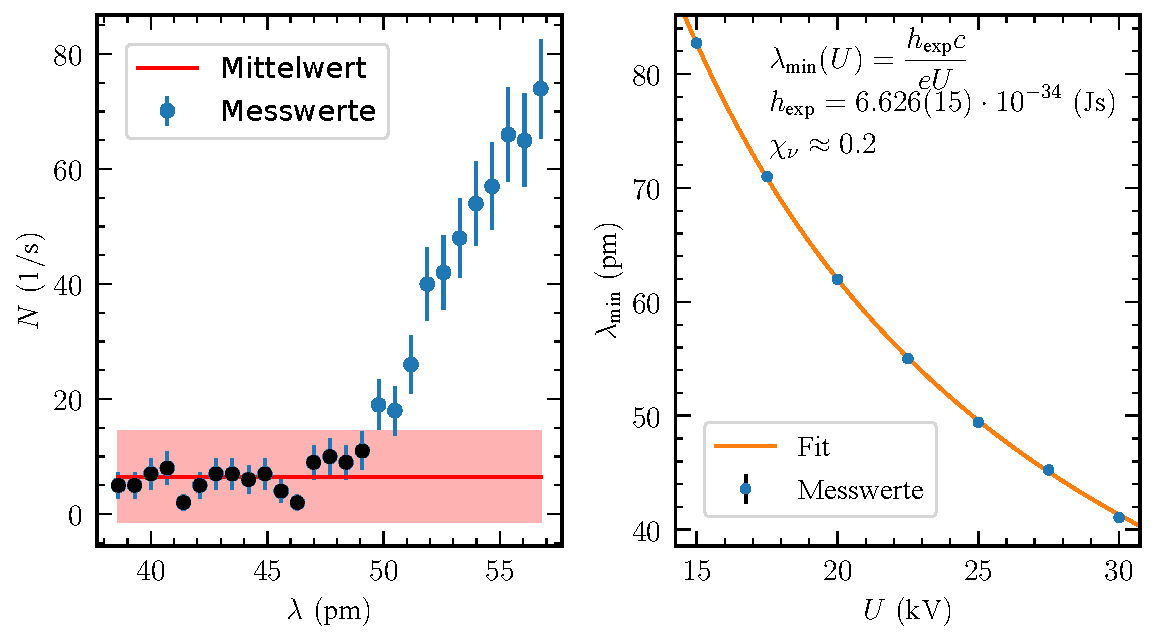
\includegraphics[width=\textwidth]{Ex3}
	\caption{\textbf{Links} ist exemplarisch die Bestimmung von \( \lambda_{\text{min}} \) dargestellt. Dabei wurde der Mittelwert der Daten im konstanten Bereich (Datenpunkte sind rot markiert) berechnet und mit einem \( 3\sigma \) Fehlerband bestückt. \( \lambda_{\text{min}} \) liegt dann in der Mitte zwischen dem ersten Wert, welcher mehr als \( 3\sigma \) vom Mittelwert abweicht, und dem davor. \textbf{Rechts} ist \( \lambda_{\text{min}} \) auf die gesetzte Beschleunigungsspannung \( U \) aufgetragen. In orange wurde eine Funktion an alle Datenpunkte angepasst, aus welcher sich die Planck Konstante ermitteln lässt. Die \( 1\sigma \) Fehler sind nicht sichtbar, da sie zu klein sind.}
	\label{fig:Ex3}
\end{figure}

Im rechten Plot in \autoref{fig:Ex3} sieht man, dass die ermittelten \( \lambda_{\mathrm{min}} \) gut zur Theorie passen. Die Fehler von \( \lambda_{\mathrm{min}} \) wurden sogar etwas zu groß abgeschätzt, was sich im reduzierten Chi-Quadrat \( \chi_\nu \approx 0.2 \) widerspiegelt (sollte bei 1 liegen). Vergleicht man den gefitteten Wert der Planck Konstante mit dem Codata Referenzwert \autocite{codata}
\begin{equation*}
	h_{\text{exp}} = 6.626(15) \cdot 10^{-34} \unit{Js} \qquad\text{und}\qquad h_{\text{lit}} = 6.626 \cdot 10^{-34} \unit{Js},
\end{equation*}
dann treffen wir dieses im Rahmen unserer Unsicherheit.

Weiters können wir noch den Einfluss von diversen Materialien auf die Intensität der Röntgenstrahlung untersuchen. Dafür wurde Zink und Aluminium in unterschiedlichen Dicken vor den GMZ eingeführt und die Zählrate gemessen. In \autoref{fig:Ex4_1} sind die Daten dargestellt, wobei der Datenpunkt bei \( d = 0 \unit{mm} \) verwendet wurde, um die restlichen Messwerte zu normalisieren und untereinander vergleichbarer zu machen. Der erste Datenpunkt hat dann per Definition keine Unsicherheit mehr; diese fließt in die Unsicherheit der restlichen Werte ein. Die Messungen wurden bei \( \lambda = 73.4 \unit{pm} \) (blau in \autoref{fig:Ex4_1}) und \( \lambda = 104.3 \unit{pm} \) (orange) durchgeführt. Zusätzlich wurden Exponentialfunktionen der Form \( N(d)/N_0 = \exp(-\mu d) + c \) angepasst, mit dem Absorptionskoeffizienten \( \mu \) und der Hintergrundstrahlung \( c \) als freie Parameter.

\begin{figure}[H]
	\centering
	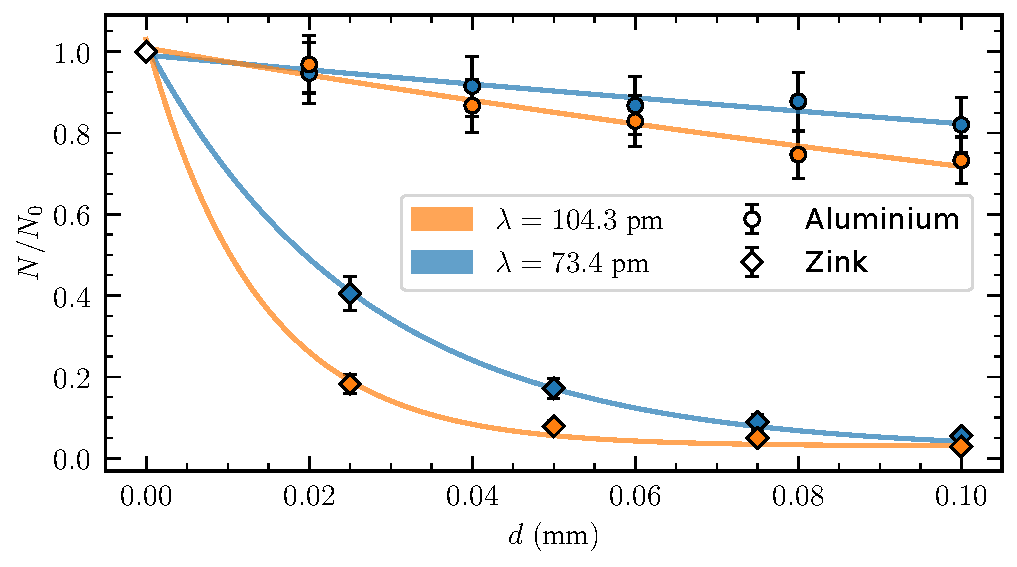
\includegraphics[width=\textwidth]{Ex4_1}
	\caption{Die Zählrate mit Absorber wurde mit der Rate ohne Absorber normalisiert \( N/N_0 \) und auf die Dicke \( d \) des Absorbers aufgetragen. Der Datenpunkt bei \( d = 0 \unit{mm} \) ist somit der Referenzwert für alle Messungen und wird ohne Fehler angegeben. Zwischen den zwei untersuchten Materialien kann man anhand der marker der Datenpunkte unterscheiden, während Messungen verschiedener Wellenlängen farblich auseinanderzuhalten sind. Zudem wurden Exponentialfunktionen der Form \( N/N_0(d) = \exp(-\mu d)+c \) angepasst und als durchgezogene Linie in der Graphik dargestellt.}
	\label{fig:Ex4_1}
\end{figure}

In \autoref{fig:Ex4_1} kann man gut erkennen, dass Zink der bessere Absorber ist und, dass die Absorption offensichtlich von der Wellenlänge (bzw. Energie) der Photonen abhängt. Teilt man den Absorptionskoeffizienten durch die Dichte des Materials, erhält man den Massenabsorptionskoeffizienten \( \mu/\rho \), welcher in NIST Datenbanken \autocite{nist_Daten} für diverse Energien zu finden ist. Um die Literaturwerte auf unsere Energien anzupassen, wurde linear interpoliert.

\begin{center}
	\captionof{table}{Die ermittelten Massenabsorptionskoeffizienten \( \mu/\rho \) für Aluminium und Zink bei zwei unterschiedlichen Energien werden Literaturwerten aus \autocite{nist_Daten} gegenübergestellt. \vspace{0.3cm}}
	\begin{tabular}{@{\extracolsep{5mm}} 
			l
			S[table-format=2(1)]
			S[table-format=2.1]
			S[table-format=3(2)]
			S[table-format=3.1]
		}
		\toprule
		& \multicolumn{2}{c}{\makecell{Aluminium}} & \multicolumn{2}{c}{\makecell{Zink}} \\
		\cmidrule(lr){2-3}\cmidrule(lr){4-5}
		{$E$ in $\oldunit{keV}$}
		&   {exp}
		&   {lit}
		&   {exp}
		&   {lit}\\
		\midrule
		\( 16.89 \) & 1.8(8) & 6.25 & 53(6) & 64.5 \\
		\( 11.89 \) & 13(3) & 19.3 & 103(10) & 175.6 \\
		\bottomrule
	\end{tabular}
	\label{table:murho}
\end{center}\vspace{0.5cm}

In Tabelle 1 werden die experimentell bestimmten Massenabsorptionskoeffizienten mit theoretischen verglichen und man erkennt, dass keine der Werte miteinander konsistent sind. Wir liegen etliche Standardabweichungen von den Literaturwerten entfernt und können nur die steigende Tendenz bei höherer Energie korrekt wiedergeben. Das könnte an Verunreinigungen der Proben liegen.

Zuletzt wird noch das Verhalten des Massenabsorptionskoeffizienten bei konstanter Dicke und unterschiedlichen Energien untersucht. Dafür wurde die Zählrate bei diversen Winkeln aufgenommen, woraus sich aus dem früheren Spektrum ohne Absorber und \autoref{eqn:mu} der Absorptionskoeffizient für jeden Datenpunkt berechnen lässt. Gemäß \autoref{eqn:tau} sollte \( \mu/\rho \propto \lambda^3 \propto 1/E^3\), falls der Photoeffekt der dominierende Streumechanismus ist. Haben die Photonen die Ionisierungsenergie eines Elektrons, dann ändert sich \( \mu \) sprunghaft, was als Absorptionskante bekannt ist. Im Falle von Kupfer und Nickel liegt eine Absorptionskante innerhalb des beobachteten Energieintervalls vor. Um die Ionisierungsenergie zu ermitteln wurde der sprunghafte Bereich isoliert (über die Änderung zwischen benachbarten Datenpunkten). \( E_K \) wurde dann auf die Mitte des Intervalls gesetzt, mit halber Breite als Unsicherheit. Ab der Absorptionskante lässt sich das charakteristische \( 1/E^3 \) Verhalten beobachten, was durch einen Fit der Form \( \mu(E)/\rho = k(Zhc/E)^3 + a \), mit Lichtgeschwindigkeit \( c \), Kernladungszahl \( Z \), konstantem Offset \( a \), Proportionalitätskonstante \( k \). In \autoref{fig:Ex4_3} ist die Auswertung exemplarisch für Kupfer dargestellt.

\begin{figure}[H]
	\centering
	\adjincludegraphics[clip, trim = {0 {.5\height} 0 0}, width=\textwidth]{Ex4_3}
	\caption{Der Massenabsorptionskoeffizient \( \mu/\rho \) ist für Kupfer auf die Energie (unten) sowie Wellenlänge (oben) aufgetragen. Ab einer bestimmten Energie \( E_K \) ändert sich das Verhalten sprunghaft. Danach lässt sich eine \( 1/E^3 \) Abhängigkeit beobachten, was durch eine Fitfunktion in Rot angedeutet wird. Substrukturen wurden aus dem Fit ausgenommen.}
	\label{fig:Ex4_3}
\end{figure}

Eine Messung mit Nickelabsorber wurde ident durchgeführt (Daten im Anhang) und wir kommen auf
\begin{align*}
	E_{\text{Cu, exp}} &= 9.3(3) \unit{keV} \qquad &E_{\text{Ni, exp}} &= 8.38(13) \unit{keV} \\
	E_{\text{Cu, lit}} &= 8.98 \unit{keV}  \qquad &E_{\text{Ni, lit}} &=8.33 \unit{keV}.
\end{align*}

Die Literaturwerte wurden aus \autocite{nist_Daten} entnommen.
Aluminium, Zinn und Zink als Absorbermaterialien wurden auch getestet, die Messintervalle sind hier aus Zeitgründen nicht mehr konsistent durchgeführt worden und unterscheiden sich sowohl in Länge als auch in Auflösung. Für Zinnober lasst sich das $1/E^3$ Verhalten gut durch einen Fit bestätigen, selbiges gilt für Aluminium, wobei die Auflösung hier schlechter ist und Substrukturen nicht mehr zu sehen sind. Bei Zink hingegen ist das Messintervall zu kurz, sodass kein sinnvoller Fit durchgeführt werden konnte.
	